\documentclass[screen, ngerman]{beamer}

\usepackage{babel}
\usepackage[utf8]{inputenc}
\usepackage[T1]{fontenc}
\usepackage{lmodern}
\usepackage{geometry}
\usepackage{graphicx}
\usepackage{amsmath}

\title{Informationsentropie}
\author{Tamara Szecsey}

\begin{document}
	\begin{frame}
		\maketitle
	\end{frame}
	
	\begin{frame}
		\tableofcontents
	\end{frame}
	
	\section{Was ist Informationsentropie?}
	\begin{frame}{Informationsentropie}
		Die Entropie zählt wieviele Mikrozustände eines Systems einen Makrozustand bilden. 
		
		Beispiel: Wurf von zwei W6 Würfeln. 
		
		Wie viele Ja-Nein-Fragen muss man beantworten, um das Ergebnis zu bekommen?
		
		Beispiel: Münzwurf hat die Informationsentropie von 1 Bit.
%		\begin{figure} [h] 
%			\begin{center}
%				\includegraphics[width=0.5\textwidth]{Information}
%			\end{center}
%		\end{figure} 		
	\end{frame}
	
	\section{Die drei Hauptsätze}
	\begin{frame}{Der Nullte Hauptsatz der Thermodynamik}	
%		\begin{figure} [h] 
%			\begin{center}
%				\includegraphics[width=0.5\textwidth]{Verschraenkung}
%			\end{center}
%		\end{figure} 	
%		\begin{figure} [h] 
%			\begin{center}
%				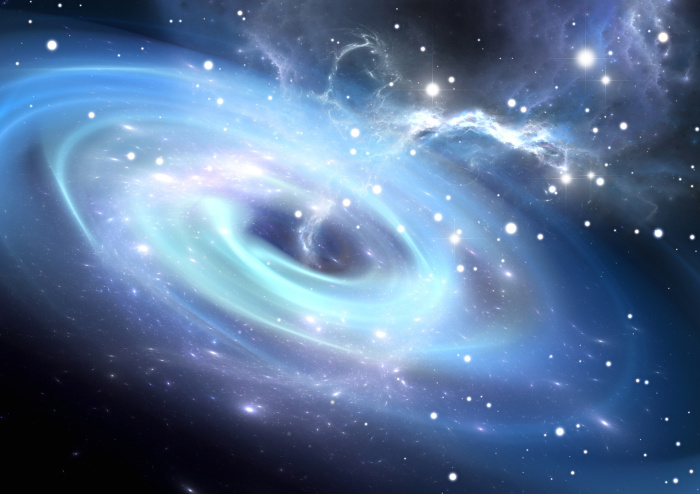
\includegraphics[width=0.5\textwidth]{Hawkingstrahlung}
%			\end{center}
%		\end{figure} 		
	\end{frame}
	
	\begin{frame}{Der Erste Hauptsatz der Thermodynamik}
%		\begin{figure} [h] 
%			\begin{center}
%				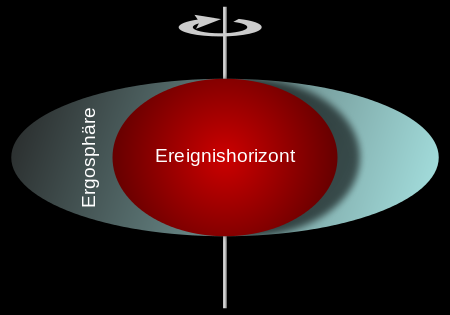
\includegraphics[width=0.5\textwidth]{Kerr-Neumann}
%			\end{center}
%		\end{figure} 		
	\end{frame}	

	\begin{frame}{Der Zweite Hauptsatz der Thermodynamik}
		\begin{figure} [h] 
			\begin{center}
				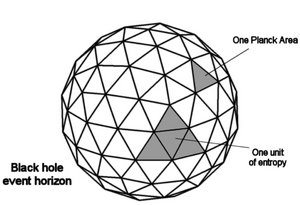
\includegraphics[width=0.5\textwidth]{BHentropy1}
			\end{center}
		\end{figure}
%		\begin{figure} [h] 
%			\begin{center}
%				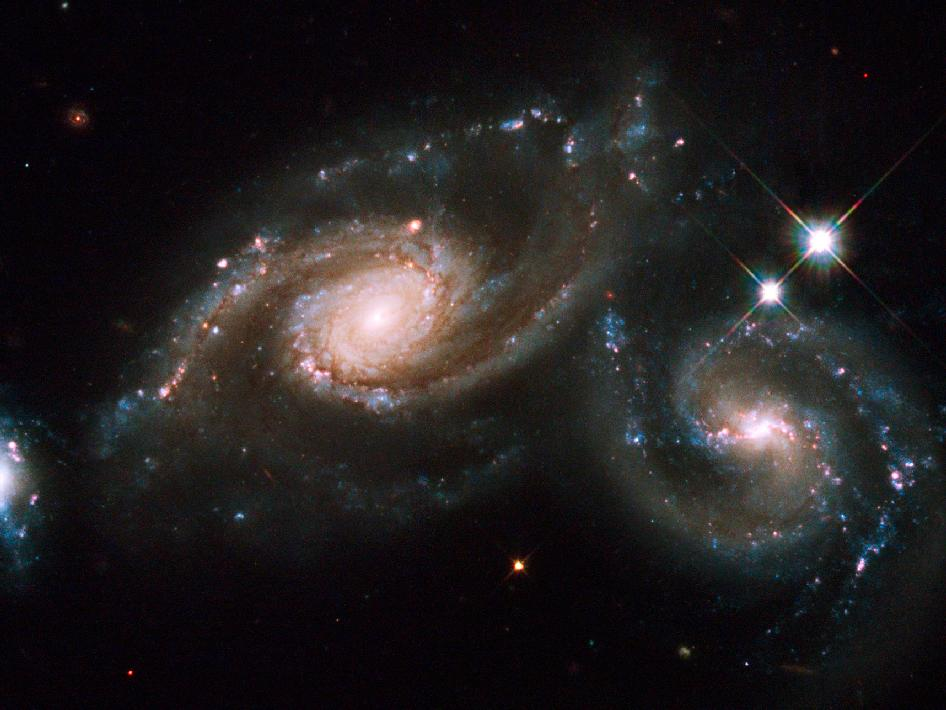
\includegraphics[width=0.5\textwidth]{kollidierendeSHs}
%			\end{center}
%		\end{figure}  
	\end{frame}
	
	\section{Verdampfung}
	\begin{frame}{Verdampfung/Evaporation}
%		\begin{figure} [h] 
%			\begin{center}
%				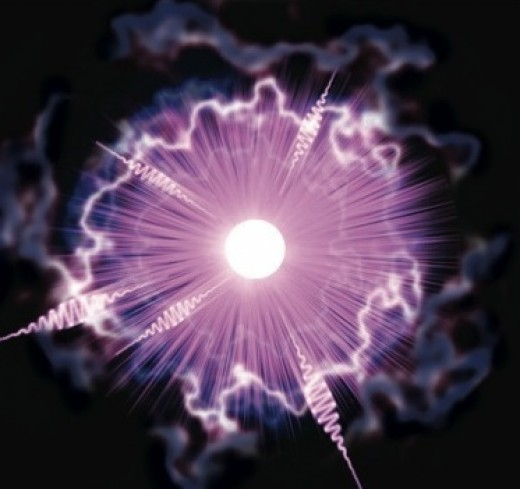
\includegraphics[width=0.5\textwidth]{evaporation}
%			\end{center}
%		\end{figure} 
	\end{frame}
	
	\section{Weitere Betrachtung}
	\begin{frame}{Weitere Betrachtung}
%		\begin{figure} [h] 
%			\begin{center}
%				\includegraphics[width=0.5\textwidth]{weisses_schwarzes_Loch}
%			\end{center}
%		\end{figure} 
	\end{frame}	
\end{document}